\documentclass{article}
\usepackage{graphicx} % Required for inserting images
\usepackage{float}
\graphicspath{ {./images/} }

\title{EP2 - MAP2220 - Analise Numérica}
\author{\\ \\
        Rennisson Davi D. Alves \\%
        NUSP 13687175
        \\ \\}
        
\date{Novembro 2023}

\begin{document}

\maketitle

\section{Introdução}
    \paragraph{} Aqui neste trabalho estudaremos as aproximações racionais de Padé,
    dada uma função f(x) e dois inteiros m e n tais que m + n = N.

    Para tal estudo, implementamos um algoritmo em Python (versão 3.10) para que,
    dadas as características de f(x) e dois inteiros m e n, sejamos capazes de
    estimar um polinômio do tipo

    \begin{equation}
        r(x) = \frac{p(x)}{q(x)} = \frac{p_{0} + p_{1}x + p_{2}x^{2} + ... + p_{n}x^{n}}{q_{0} + q_{1}x + q_{2}x^{2} + ... + q_{m} x^{m}}
    \end{equation}
    onde p(x) tem grau n e q(x) tem grau m.

    Nota para alguns abusos de notação: utilizei o formato de tupla (m, n) para denotar os grau de p(x) e q(x) por m e n, respectivamente.
    
    Sobre os gráficos, na cor preta está o gráfico da função objetiva f(x). Em linhas pontilhadas vermelhas, está o gráfico de $P_{N}(x)$,
    que é o polinômio de MacLaurin. Finalmente, em linhas pontilhadas verdes está o gráfico de r(x).

\section{O Algoritmo}

    \paragraph{} Como referência, utilizamos o algoritmo 8.1 presente no capítulo 8 do livro
    \textit{Numerical Analysis}, dos autores Richard L. Burden e J. Douglas Faires.
    Para a resolução do sistema linear, substituímos a que está presente no algoritmo citado
    e utilizamos o módulo \textit{linalg} da biblioteca \textit{Numpy}.

    Dois fatores nos levaram para essa substituição no código original.
    Na primeira implementação do código os coeficientes dos polinômios P e Q não estavam
    corretos. Seus valores diferiam dos valores que foram encontrados quando fizemos os cálculos
    na mão. Na tentativa de consertar o código, acabamos por nos confundir ainda mais com os
    índices dos arrays de entrada e saída.

    O segundo fator tem a ver com a redução de linhas de código digitadas. Economizando tempo
    na hora de programar (um trecho de algoritmo que tinha aproximadamente 30 linhas foi 
    substituído por outro que tem 3 linhas) e garantindo os resultados corretos da resolução
    do sistema linear, já que a biblioteca \textit{Numpy} foi amplamente testada e otimizada para melhor precisão.

    Apesar da troca do algoritmo, um erro ainda persistiu. Este que impedia uma boa aproximação da
    função objetiva através do polinômio racional de Padé. Após outra revisão no código, foi encontrado o erro e o algoritmo finalmente chegou em sua versão final, com resultados
    mais refinados.

    A biblioteca \textit{Simpy} também foi muito útil neste trabalho.
    Seu encargo era guardar as funções desejadas de maneira "simbólica", calcular suas
    derivadas de ordem n e retornar o valor das funções em um dado ponto x.
    Seu uso se deu principalmente quando o objetivo era encontrar os coeficientes do polinômio
    de MacLaurin (polinômio da Taylor quando x = 0), visto que seria necessário calcular
    diversas derivadas que a cada iteração aumentavam sua ordem.
    Ao derivas as funções, substituíamos o valor de x por zero e encontravámos o coeficiente i do polinômio de MacLaurin.


\section{Testes}
    Para avaliar as aproximações racionais de Padé, foi pedido que verificássemos a norma do máximo $\left | f(x) - g(x) \right |$
    e a norma de $\l^{2}$ dentro do intervalo [0, 1]. Além disso, foi fixado N = 6. Desse modo,
    testamos todas as combinações possíveis para m e n tais que m + n = 6.
    Ou seja, para cada função nós geramos 7 aproximações racionais de Padé.

    
    O primeiro teste realizado foi com a função f(x) = $e^{x}\cos{x}\sin(x)$ definida já no enunciado deste EP.
    Abaixo está uma tabela com os resultados obtidos dos testes:
    
    \begin{table}[h]
        \centering
        \caption{f(x) = $e^{x}\cos{x}\sin(x)$}
        \label{tab:my_table}
            \begin{tabular}{|c|c|c|c|c|} \hline 
                 (m, n)&  $\left | f(x) - P_{6}(x) \right |$&  $\l^{2}$&  $ \left |f(x) - r(x) \right |$& $\l^2$\\ \hline 
                 (0, 6)&  0,030307&  0,432747&  0,030307& 0,437293\\ \hline 
                 (1, 5)&  0,030307&  0,432747&  0,035250& 0,436509\\ \hline 
                 (2, 4)&  0,030307&  0,432747&  0,012708& 0,444426\\ \hline 
                 (3, 3)&  0,030307&  0,432747&  107,177744& 107,477285\\ \hline 
                 (4, 2)&  0,030307&  0,432747&  0,088816& 0,459684\\ \hline 
                 (5, 1)&  0,030307&  0,432747&  0,462249& 0,736880\\ \hline 
                 (6, 0)&  0,030307&  0,432747&  0,030307& 0,437293\\ \hline
            \end{tabular}
    \end{table}

    Como vemos neste exemplo, a menor norma $\l^2$ foi para r(x) com m = 1 e n = 5, que é 0,436509.
    Já quando chegamos em m = 2 e n = 4, encontramos a menor norma do máximo, que assume o valor 0,012708.
    No geral, essa foi mesmo a função que melhor se aproximou da função original, junto com o próprio
    polinômio de MacLaurin e o polinômio r(x) quando m = 2.

    Agora, para m = n = 3, apresentou-se uma anomalia na aproximação de Padé.
    Quando $x \in (0.70, 0.75)$ a função r(x) se afasta drasticamente de f(x), tanto que em x = 0.722408
    ambos os erros calculados chegam a ultrapassar o valor de 105. Analiticamente, quando x tende para um valor próximo
    de 0.72 (seja pela esquerda ou pela direita), a função r(x) tende para o infinito com uma curva assintótica que lembra
    a exponencial.
    
    Abaixo deixaremos alguns gráficos que ilustrarão as aproximações. Respectivamente, estão os gráficos para
    (m, n) = (0, 6), (m, n) = (2, 4), (m, n) = (1, 5) e para (m, n) = (3, 3). Este último que mostrará a anomalia
    do polinômio r(x) quando m = n = 3.
    
    \begin{figure}[h]
        \centering
        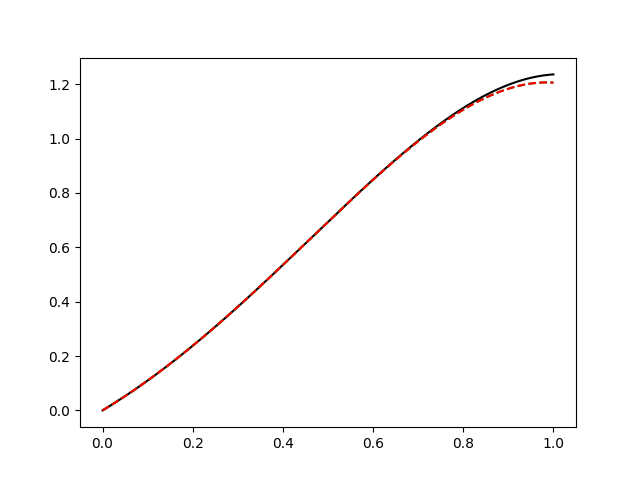
\includegraphics[width=0.45\textwidth]{Figure_2.png}
        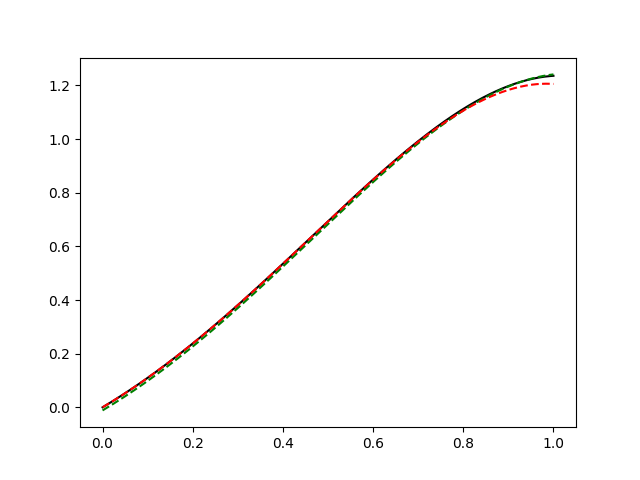
\includegraphics[width=0.45\textwidth]{Figure_3.png}\\
        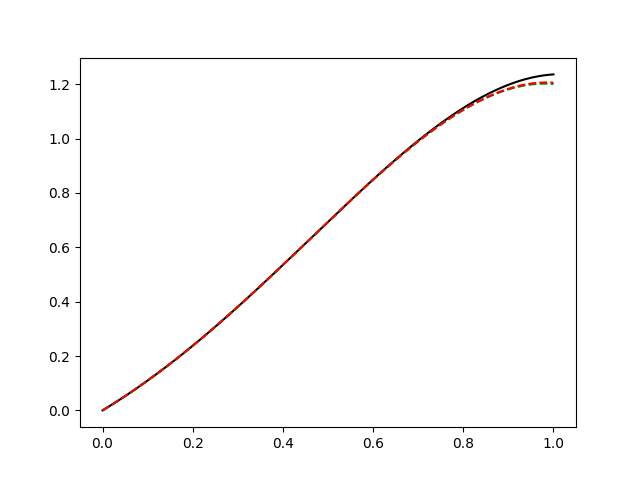
\includegraphics[width=0.45\textwidth]{Figure_8.png}
        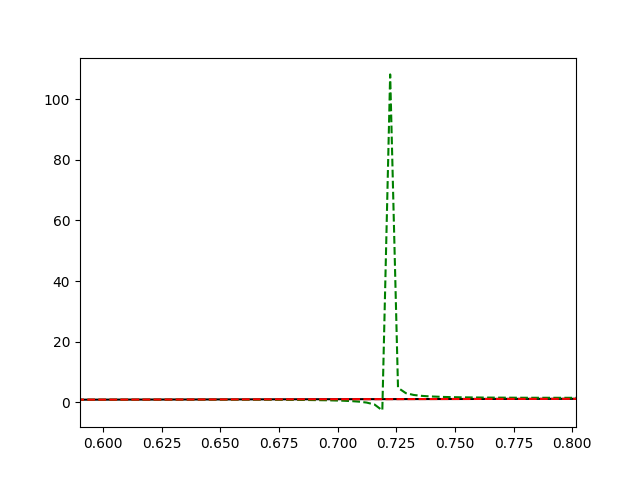
\includegraphics[width=0.45\textwidth]{Figure_1.png}\\
    \end{figure}

    O segundo teste realizado foi com uma função arbitrária de nossa escolha.
    Como requisito, ela deveria ser uma combinação de multiplicações, divisões
    e potências de $e^{x}$, $\cos{x}$ e $\sin{x}$.
    A função escolhida foi f(x) = $\frac{\sin(x)\cos^{2}{x}}{e^{x}}$.
    Abaixo está uma tabela com os resultados obtidos dos testes:

    \begin{table}[h]
        \centering
        \caption{f(x) = $\frac{\sin(x)\cos^{2}{x}}{e^{x}}$}
        \label{tab:my_table2}
            \begin{tabular}{|c|c|c|c|c|} \hline 
                 (m, n)&  $\left | f(x) - P_{6}(x) \right |$&  $\l^{2}$&  $ \left |f(x) - r(x) \right |$& $\l^2$\\ \hline 
                 (0, 6)&  0,11259&  1,44564&  0,112590& 1,368344\\ \hline 
                 (1, 5)&  0,11259&  1,44564&  0,246810& 1,125504\\ \hline 
                 (2, 4)&  0,11259&  1,44564&  0,013225& 1,277095\\ \hline 
                 (3, 3)&  0,11259&  1,44564&  0,0450831& 1,318677\\ \hline 
                 (4, 2)&  0,11259&  1,44564&  0,007938& 1,280812\\ \hline 
                 (5, 1)&  0,11259&  1,44564&  0,042374& 1,256806\\ \hline 
                 (6, 0)&  0,11259&  1,44564&  ------& ------\\ \hline
            \end{tabular}
    \end{table}

    Aqui, o menor erro quadrático vale 1,125504 para m = 1 e n = 5. Apesar de ser o menor erro quadrático, essa função
    não é uma boa aproximação. A partir de x = 0,4, r(x) vai se afastando da função objetiva.
    
    E o menor erro máximo, para m = 4 e n = 2, que vale 0,007938. Nesse caso, a função r(x) se aproxima bastante da função
    f(x) = $\frac{\sin(x)\cos^{2}{x}}{e^{x}}$ em todo o intervalo [0, 1]. Trata-se então da melhor aproximação encontrada.
    
    Quando fazemos m = 6, o algoritmo não foi capaz de encontrar os coeficientes de p(x) e q(x), por se tratar de uma
    matriz singular. Portanto, afirma-se que neste caso não há um polinômio do tipo $\frac{p(x)}{q(x)}$, onde q(x) tem grau m = 6, que se aproxime de f(x).
    
    Abaixo estão os gráficos de r(x) na ordem em que foram citados neste parágrafo. Os outros dois gráficos se tratam de (m, n) = (3, 3)
    e (m, n) = (5, 1).

    \begin{figure}[h]
        \centering
        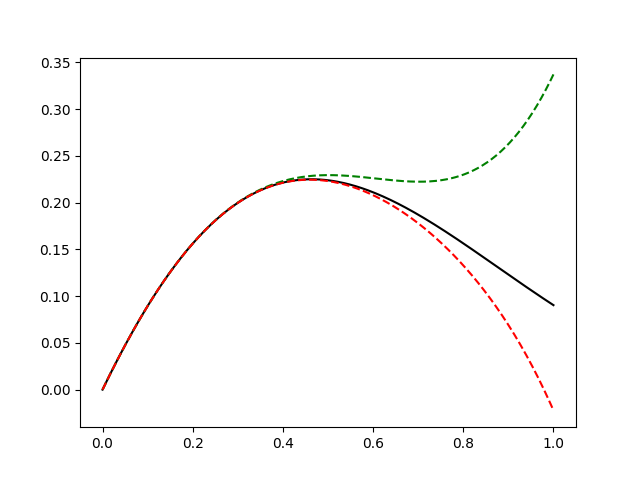
\includegraphics[width=0.45\textwidth]{Figure_4.png}
        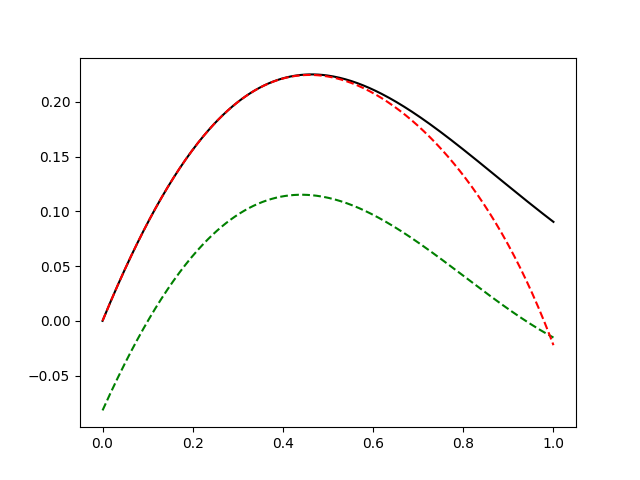
\includegraphics[width=0.45\textwidth]{Figure_5.png}\\
        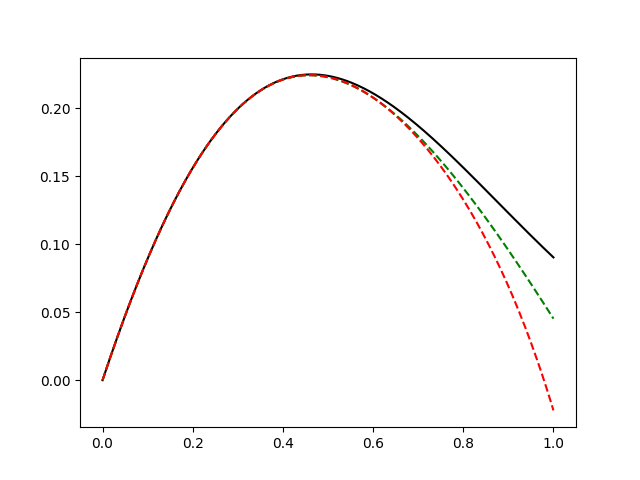
\includegraphics[width=0.45\textwidth]{Figure_6.png}
        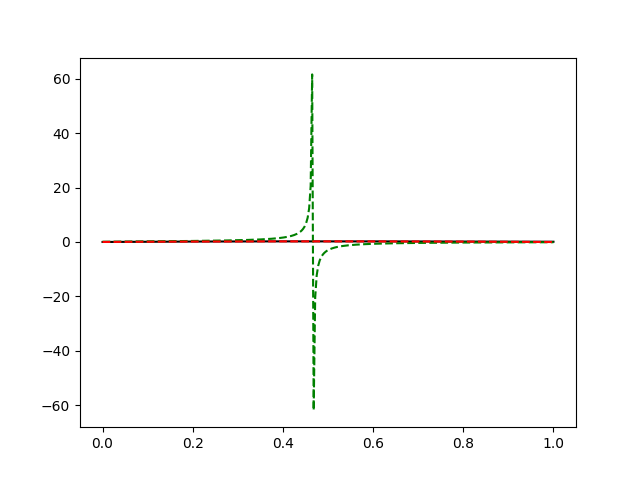
\includegraphics[width=0.45\textwidth]{Figure_7.png}\\
    \end{figure}

\section{Conclusão}

    Seguindo o que os resultados nos mostraram, as aproximações racionais de Padé
    não parecem um bom método para aproximação de funções que sejam composições de senos e cossenos
    Talvez sua forma racional aumente sua sensibilidade em certos intervalos, como foi o caso das
    anomalias apresentadas nos dois exemplos.

    A ideia de deixar m e n mais proximos para diminuir a oscilação da função parece confortável,
    mas não é exatamente isso que vemos nestes exemplos.
    O polinômio r(x) fica próximo da função objetivo mas em algum ponto do intervalo de domínio,
    r(x) começa a se afastar cada vez mais de f(x).
    
    Além disso, as tabelas e a análise dos gráficos deram a impressão de que,
    quanto maior o grau do polinômio q(x) (que está no denominador de r(x)),
    mais afastada a função r(x) fica de f(x). Ou seja, a medida que aumentamos o valor de m
    (e consequentemente n se aproxima de zero), perdemos precisão na aproximação da função.
    Quando o grau do denominador aumenta, temos menos controle sobre seus resultados.
    No segundo segundo exemplo, quando assumimos f(x) = $\frac{\sin(x)\cos^{2}{x}}{e^{x}}$,
    para m = N = 6, a matriz se torna singular, portanto não conseguimos aproximar f(x) através de um polinômio
    com grau máximo no denominador.

    Outro ponto observado: enquanto procurava uma função adequada que combinava produtos, divisão e potências de
    $e^{x}$, $\cos{x}$ e $\sin{x}$, os testes preliminares mostraram que é bem difícil aproximar essas funções utilizando
    as aproximações racionais de Padé.
    Principalmente se considerarmos que é mesmo esperada uma variação na acurácia de Padé, já que o polinômio r(x) é baseado
    na série de Taylor para $e^{-x}$. E essa mesma representação do polinômio de Taylor para $e^{-x}$ tem uma variação substancial
    para todo x pertencente ao intervalo [0.2, 1].

    Ainda assim, na maior parte dos casos estudados, o polinômio de Padé se mostra melhor que o polnômio de MacLaurin.
    Principalmente quando f(x) tem um denominador diferente de 1, como no segundo caso que estudamos, o Padé respondeu
    melhor e se aproximou mais de f(x), exceto quando definimos m = 1.

    
\end{document}
